\chapter{Úvod}

\todo{reference na kapitoly ..ref..}

Zpracování řeči hraje v dnešní době důležitou roli v mnoha rozličných oborech. Mezi jedny z hlavních úkolů bezesporu patří separace zdrojů v nějakém zaznamenaném signálu, který může být složen ze signálů N mluvčích, ale i nechtěného hluku okolí. Vyřešení problému je předpoklad k dalším úkonům jako identifikace konkrétního mluvčího nebo třeba přepis nějaké konverzace na text. Se stále se zrychlujícím vývojem počítačů a s jejich zvyšujícím se výkonem se do popředí dostávají metody zpracování řeči založené na neuronových sítích, které v mnoha ohledech předčily doposud používané algoritmy.

Separace mluvčích v časové doméně dosahuje mimořádných výsledků v porovnání s dosavadními metodami LSTM založenými na převodu signálu z časové domény do frekvenční domény. Taková reprezentace signálu není optimální pro udržení časových závislostí, které jsou při zpracování řeči podstatné. V referenční studii je vstupní signál převeden do nezáporné reprezentace, která je optimální pro extrakci jednotlivých mluvčích. Silnou stránkou systému je hluboká architektura sítě, která lépe modeluje dlouhodobé závislosti v signálu.

Téma v oblasti neuronových sítí jsem si vybral, jelikož ty zažívají obrovský rozmach a pomalu se stávají součástí téměř všech odvětví a tudíž je velmi perspektivní pro další výzkum. Právě bakalářskou práci jsem vyhodnotil jako dobrou příležitost k seznámení se s neuronovými sítěmi a vyzkoušení si, jak se s nimi pracuje, jak se implementují modely za pomoci frameworku a jak náročná je aplikace na nějaký reálný problém.

Mým úkolem v rámci práce je nastudovat si problematiku neuronových sítí a jejich základní principy, seznámit se problémem separace mluvčích pomocí neuronových sítí a následně implementovat síť podle architektury TasNet pro separaci mluvčích v časové doméně, která byla navržena a popsána ve studii\ref{referencni_studie}. Potom tuto neuronovou síť natrénovat s různými kombinacemi hodnot hyperparametrů, které ovlivňují velikost sítě a její vlastnosti, a nakonec porovnat přesnost a kvalitu separace mezi jednotlivými, různě velkými sitěmi a mezi výsledky studie. Přesnost separace je vypočítána pomocí míry si--snr, udávající poměr mezi chtěným signálem a hlukem na pozadí. Sítě budou testovány a vyhodnocovány na testovací množině jednokanálových směsí dvou mluvčích.

6) struktura prace - popsat kapitoly
\todo{prepsat podle novejch kapitol co jsem navrhoval - doplnit popsani datasetu}
V první části práce jsou popsány základní prvky neuronových sítí, struktura umělého neuronu, jeho vstupy a výstupy, váhy a role aktivační funkce. V návaznosti na to je popsán proces učení neuronových sítí. Proces učení se skládá z několika souvisejících částí, které zahrnují výpočet výstupu neuronové sítě metodou feed forward, který transformuje vstupní vektor dat a počítá na základě něj výstupní vektor, který je předán zase další vrstvě a takto analogicky až do výstupní vrstvy. Dále je rozebrán výpočet chyby, která vzniká během procesu učení, metodou gradient descent a nakonec úprava vah neuronů metodou backpropagation (zpětná propagace chyby), která se počítá na základě rozdílu mezi vstupními hodnotami a očekávánými výstupními hodnotami.
\todo{Nejsem si jistej, jestli tohle je dobre s tim backprop atd, mam dojem ze backprop pocita gradienty, a ze obj funkce pocita chybu.}

Po vysvětlení základních principů je navázáno konvolučními neuronovými sítěmi, které jsou založeny na konvoluční operaci. Konvoluční sítě se používají nejčastěji pro zpracování obrazu kvůli vlastnostem, které umožňují extrahovat příznaky s různou úrovní složitosti od základních útvarů jako úsečka, barva a podobně až po komplexnější příznaky jako část obličeje -- ucho, nos, či úplně celý obličej. Tohoto lze využít i při zpracování zvuku, kde jsou tyto extrahované příznaky jednorozměrné.

Se znalostí principu konvolučních sítí je představen konvoluční auto-enkodér, který převádí vstupní nahrávku směsi mluvčích na reprezentaci optimální pro separaci jednotlivých mluvčích.

Druhá část je věnována architektuře TasNet. V této kapitole je popsána podoba separačního modulu, jeho stavební bloky a princip. Postupně je znovu zmíněn konvoluční auto-enkodér, u nějž je vysvětlen jeho úkol v separačním modulu a následně konvoluční blok, který se sám sestává z konvolučních vrstev, normalizací a aktivačních funkcí. Tyto bloky jsou skládány za sebe se zvyšující se časovou dilatací a tvoří jádro separačního modulu.

Třetí kapitola se zabývá implementací neuronové sítě a jejím trénováním. Je popsána a zdůvodněna volba frameworku, implementace sítě a struktura zdrojového kódu. Pro usnadnění často se upakujících úkonů jsem vytvořil pár pomocných scriptů, které jsou zde také popsány. 
Model prošel během implementace několika úpravami. Pro účely trénování a validace byly vstupní nahrávky rozdělovány na čtyřsekundové segmenty. Pro testování byly používány nahrávky celé. V této kapitole je popsán průběh trénování sítí, výsledky a použité stroje a nástroje.

V poslední části jsou shrnuty experimenty s modelem - rychlost učení, vliv hyper-parametrů na učení sítě, na výsledky a přesnost výstupu v závislosti na zvolených parametrech, optimalizacích a počtu konvolučních bloků a pod. Výstup sítě v podobě separovaných mluvčích je porovnán s referenční studií.
\todo{Zminit zde taky sisnr hodnoceni a pod.}

%----------------------------------------------------------------------------------------------------------------------------------------------------------------------
\todo {Teorie: Co bylo potreba nastudovat;; uvod do problematiky;; pisu to pro nekoho, kdo chce vychazet z me bakalarky.}

\chapter{Separace mluvčích}
\label{separacemluvcich}
- obecne o problemu separace; prostredi a vyuziti, coctail party, multispeech

\chapter{Neuronové sítě}
\label{neuronovky}
body: co vlastne resi . skladaji se ze vstupni vrstvy, N skrytych vrstev, vystupni vrstvy
Co resi neuronove site.

V dnešní době zažívají neuronové sítě díky výkonosti počítačů velký rozmach. Jejich využití prostupuje skrze mnohé vědní obory a nově dokáže řešit celou řadu problémů, ve kterých dosahuje výborných výsledků, které zdaleka předčily dosavadní postupy. Mezi nejčastější úlohy, na které se neuronové sítě používají, jsou klasifikační úlohy, rozpoznávání obrazu a řeči či vzorů na videu nebo ve zvuku až po generování textu. Na základně řešeného problému vzniklo mnoho druhů neuronových sítí, z nichž některé zde budou představeny.

Nejzákladnější neuronová síť je vícevrstvá neuronová síť, neboli MLP (Multi Layer Perceptron). Tento typ sítě je skládá ze třech typů vrstev. Vstupní vrstva slouží k předání hodnot do sítě. Tato vrstva nijak nemodifikuje vstupní hodnoty, které jsou do sítě předávány a nezměněné je kopíruje první skryté vrstvě. Každá vrstva se může skládat z $1$ až $N$ neuronů, kde $N \in N$. Poslední skrytá vrstva je napojena na výstupní vrstvu. Výstupní vrstva má obvykle méně neuronů než předešlé vrstvy a hodnoty na výstupu mohou představovat třídy, do kterých má být zařazen vstup. S počtem jednotlivých vrstev souvisí pojem hloubka sítě, která je rovna počtu všech vrstev neuronové sítě od vstupní až po výstupní vrstvu.

Takto propojené neurony tvoří acyklický graf, který počítá a následně předává hodnoty směrem od vstupní vrstvy skrze skryté vrstvy až k vrstvě výstupní. Nenacházejí se zde žádná zpětná spojení, ve kterých by se výstup vracel zpět do sítě.\cite{mitdeeplearning}

Cílem takové neuronové sítě je aproximovat nějakou funkci $f^\ast$. Síti je předána vstupní hodnota $x$ a výstupní hodnota $y^\ast = f^\ast(x)$ má být co nejblíž hodnotě $y = f(x)$.


\section{Umělý neuron}
Základní stavební jednotka neuronových sítí je neuron, nebo přesněji perceptron. Tento model je založen na reálných poznatcích o neuronech, které se nacházejí v organizmu. Perceptron obsahuje libovolně mnoho vstupních synapsí, přes které se neuronu předá vstupní hodnota, váhy a jeden výstup, jehož hodnota závisí na vstupních hodnotách, vnitřním stavu neuronu (hodnoty vah a biase) a zvolené aktivační funkci. Vstupní hodnoty jsou váhovány, což v praxi znamená, že každá vstupní hodnota je vynásobena s váhou daného vstupu. Váhy v perceptronu představují nějaký vektor vah $w = [w_1, w_2, \dots, w_n]$, se kterým je vynásobený vektor vstupních hodnot $x = [x_1, x_2, \dots, x_n]$.

\todo{obrazek neuronu a popis}
\begin{figure}[H]
    \centering
    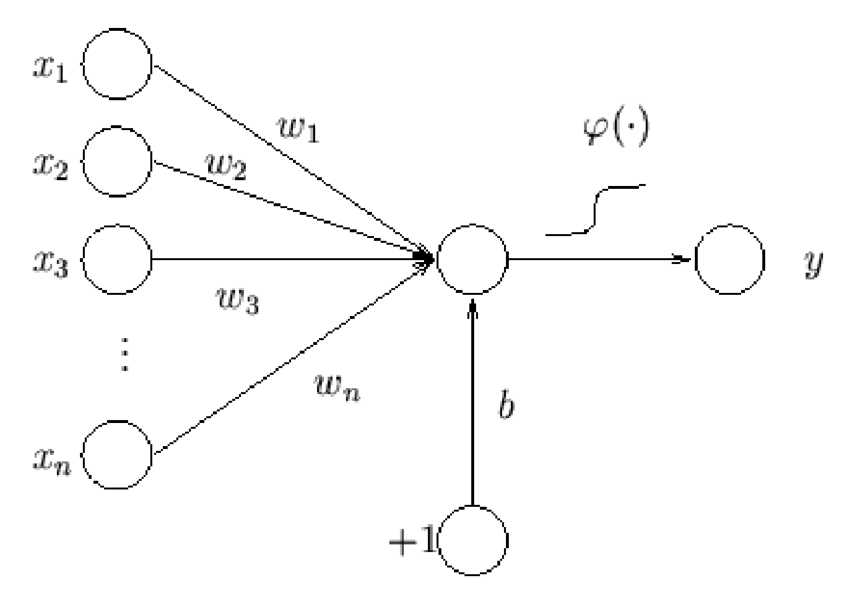
\includegraphics[scale=0.5]{obrazky-figures/perceptron.png}
    \caption{\label{fig:neuron}Schéma umělého neuronu -- perceptron}
\end{figure}

Hodnota bias $b \in R$, která je přičtena k sumě násobků vah a vstupních hodnot, modifikuje dobu, kdy se aktivuje perceptron a změní svůj výstup. Je to prahová hodnota, na základě níž je měněn výstup. Matematicky to znamená, že s aktivační funkcí horizontálně pohybuje doleva nebo doprava v závislosti na tom, je-li bias pozitivní nebo negativní. Bias se učí zároveň s ostatními váhami během učícího procesu.

\begin{figure}[H]
    \centering
    
\includegraphics[scale=1]{obrazky-figures/placeholder.pdf}
    \caption{\label{fig:bias}Vliv hodnoty bias na aktivační funkci}
\end{figure}

Výstup neuronu se vypočítá jako:
\begin{equation}
y = a((\_sum{n=1} w_nx_n) + b)
\end{equation}
kde $a$ je nějaká aktivační funkce, $x_n \in R$ je vstupní hodnota, $w_n \in R$ je váha, kterou se vstupní hodnota vynásobí a $b \in R$ je hodnota bias, která je přičtena k celkové sumě předtím, než se výsledek předá aktivační funkci.


\section{Aktivační funkce}
Aktivační, neboli prahová funkce určuje výstupní hodnotu neuronu. Funkce se vybírá na základě problému, který se má neuronová síť naučit řešit. Správná volba prahové funkce vede k lepší konvergenci učení sítě. Naopak špatná volba může vést ke stále větší odchylce od správného řešení -- může divergovat. Povaha problému může vyžadovat specifické vlastnosti aktivační funkce - lineární nebo nelineární -- sigmoidní a podobně. Pro správnou volbu aktivační funkce je pro nestandardní problémy potřeba experimentálně zjistit, která bude nejlépe vyhovovat.

\subsection*{Sigmoid}
\begin{equation}
  f(x) = \frac{1}{1+\exp(-z)}
\end{equation}
\blindtext{1}
\begin{figure}[H]
    \centering
    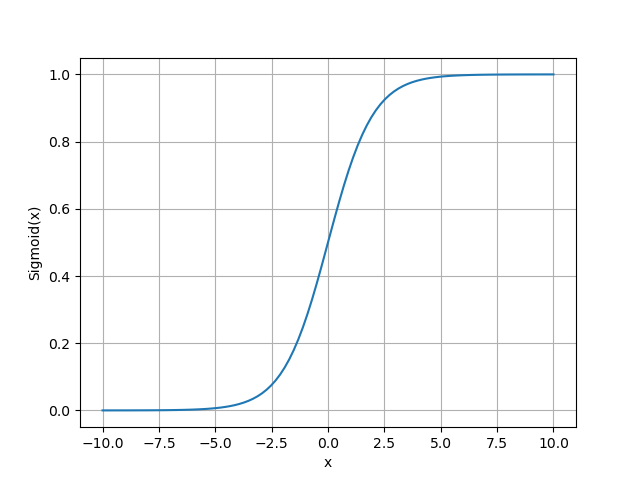
\includegraphics[scale=0.2]{obrazky-figures/sigmoid.png}
    \caption{\label{fig:sigmoid}Graf aktivační funkce sigmoid}
\end{figure}

\subsection*{Softmax}
\begin{equation}
  f(x) = \frac{1}{1+\exp(-z)}
\end{equation}
\blindtext{1}
\begin{figure}[H]
    \centering
    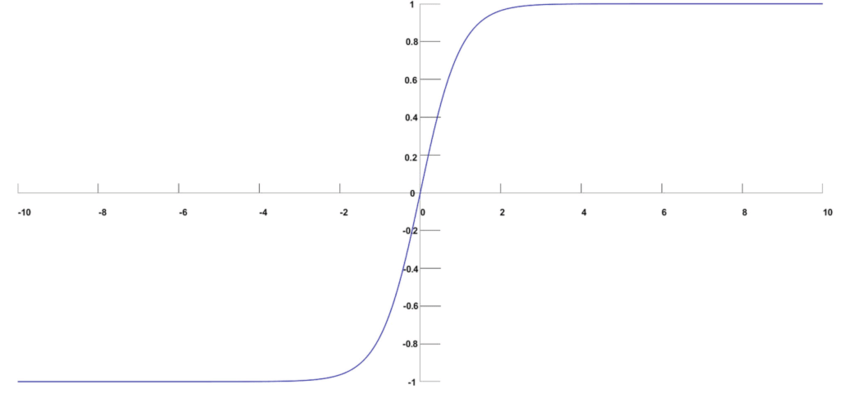
\includegraphics[scale=0.2]{obrazky-figures/softmax.png}
    \caption{\label{fig:softmax}Graf aktivační funkce softmax}
\end{figure}

\subsection*{ReLU}
Rectified Linear Unit je nejčastěji používaná aktivační funkce. Vyžaduje-li neuronová síť nějakou nelinearitu, je RelU pro většinu případů ideální. Pro každou zápornou hodnotu $x$ vrací $0$ a pro kladnou hodnotu $x$ vrací tutéž hodnotu $x$.
\begin{equation}
   f(x)=max(0,x)
\end{equation}
\blindtext{1}
\begin{figure}[H]
    \centering
    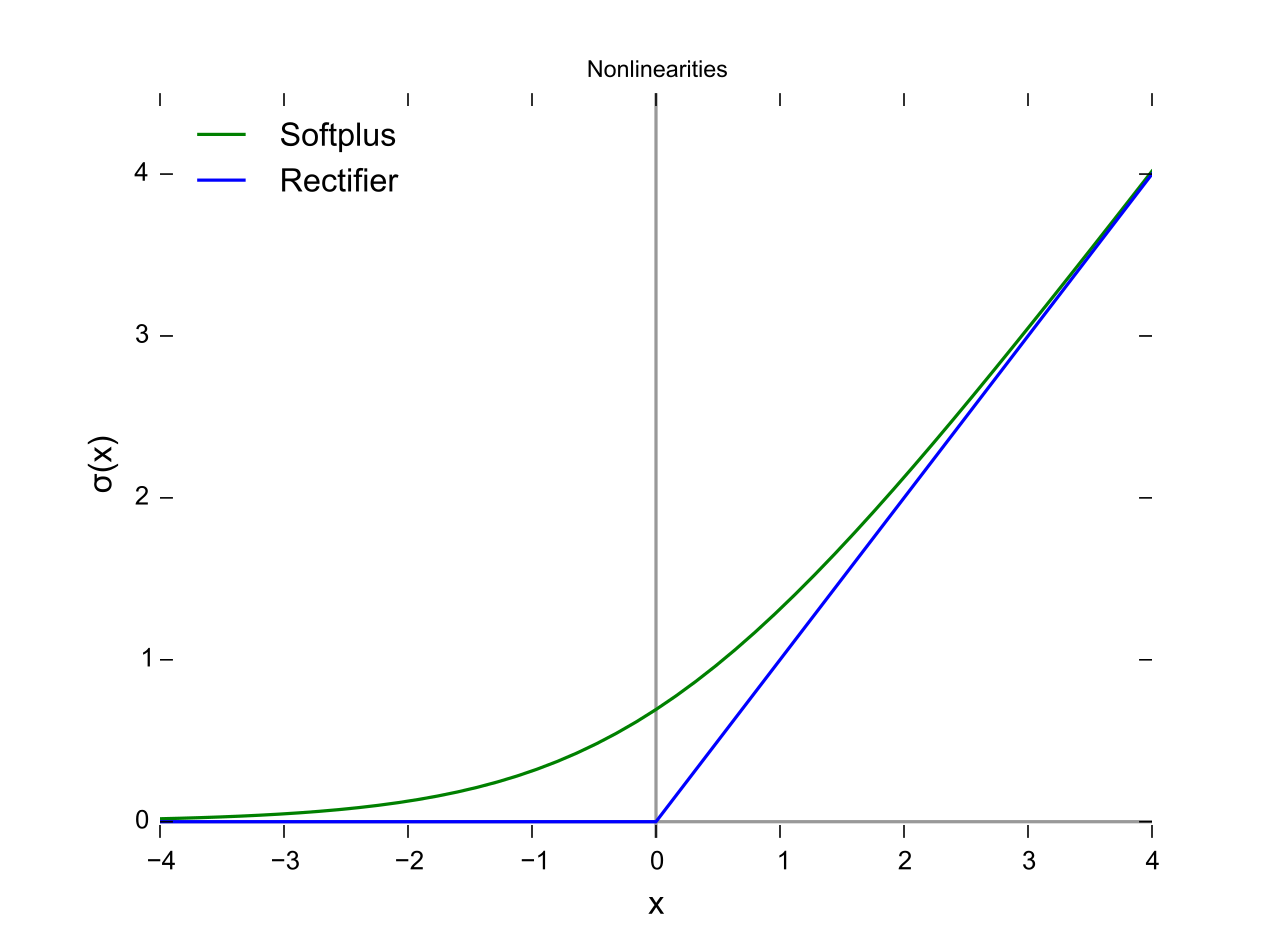
\includegraphics[scale=0.2]{obrazky-figures/ReLU.png}
    \caption{\label{fig:relu}Graf aktivační funkce ReLU}
\end{figure}


\subsection*{PReLU}
Parametrizovaná ReLU je nelineární aktivační funkce, která se používá v případě, že chceme produkovat na výstup malý nenulový gradient i v případě záporné vstupní hodnoty $x$. V tom případě je vstupní hodnota vynásobena parametrem $\alpha$ a to představuje výsledek. Parametr $\alpha$ se společně s ostatními váhami učí během učícího procesu.
\begin{equation}
  f(x) =
  \begin{cases}
    x & \text{if } x \geq 0 \\
    {\alpha}x & \text{if } x < 0
  \end{cases}
\end{equation}
\blindtext{1}
\begin{figure}[H]
    \centering
    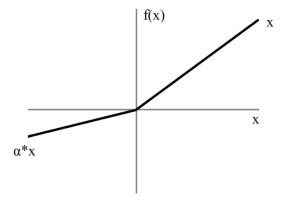
\includegraphics[scale=1]{obrazky-figures/prelu.jpg}
    \caption{\label{fig:prelu}Graf aktivační funkce PReLU}
\end{figure}



\section{Proces učení neuronových sítí}
\blindtext{1}

\subsection{Objektivní funkce}
= cost funkce
-popis, co to je, k cemu to je, proc to je...

\subsection*{MSELoss}
- vzorecek
\subsection*{Cross Entrophy}
- vzorecek

\subsection{Inicializace parametrů}
\todo{Mozna, Kniha strana 292}


\subsection{Optimalizační algoritmy}
 [1 deep learning str 301]

\subsection*{Adam}

\todo{Kniha strana 301}

Adam je jeden z algoritmů s adaptivním učením. Jeho název byl odvozen z fráze "adaptive moments".  [1 deep learning str 301]


\subsection{Backpropagation}
- zpetne sireni chyby
- adaptacni algoritmus, podil neuronu na chybe,
- 3 opakujici se faze uceni:

\todo{dodelat zde podkapitoly v lepsim poradi}

1) feedforward - dopredu
2) zpetne sireni chyby - Backpropagation
3) uprava vah a biasu na zaklade chyby
- chain rule

\blindtext{1}


\subsection*{Feed Forward}
\blindtext{1}

\subsection*{Gradient descent}
\blindtext{1}

\subsection{Overfitting a generalizace}
\blindtext{1}


\section{Konvoluční neuronové sítě}
\blindtext{1}

\subsection{Konvoluce}
\blindtext{1}


%----------------------------------------------------------------------------------------------------------------------------------------------------------------------


\chapter{TasNet - Time--Domain Audio Separation Network}
\label{tasnet}
\todo{Architektura full -- obrázek, bloky...}
\begin{figure}[H]
    \centering
    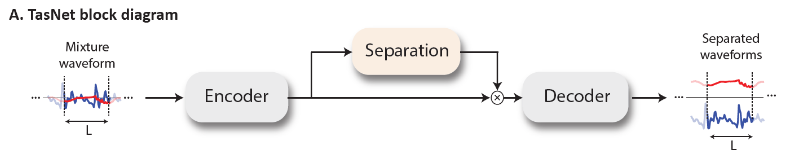
\includegraphics[scale=0.5]{obrazky-figures/tasnet-pipe.png}
    \caption{\label{fig:tasnet-pipe}Zjednodušený model architektury}
\end{figure}
\blindtext{1}

\section{Konvoluční auto--enkodér}
\todo{Konvoluční autoenkodér, vstup, výstup...}

- schema bez separacniho modulu
- non negative representation of audio
\begin{figure}[H]
    \centering
    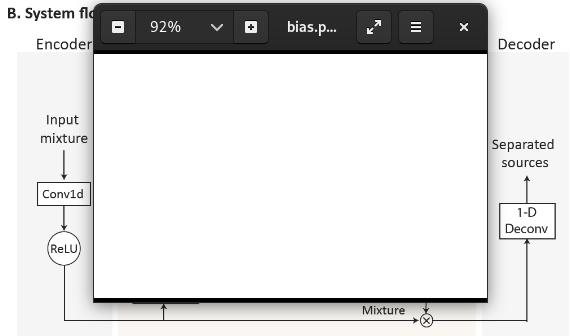
\includegraphics[scale=0.5]{obrazky-figures/tasnet-autoencoder.png}
    \caption{\label{fig:tasnet-autoencoder}Schéma konvolučního autoenkodéru}
\end{figure}
\blindtext{1}

\section{Separační modul}
- odhad masek pro jednotlive mluvci
- schema se separacnim modulem
\begin{figure}[H]
    \centering
    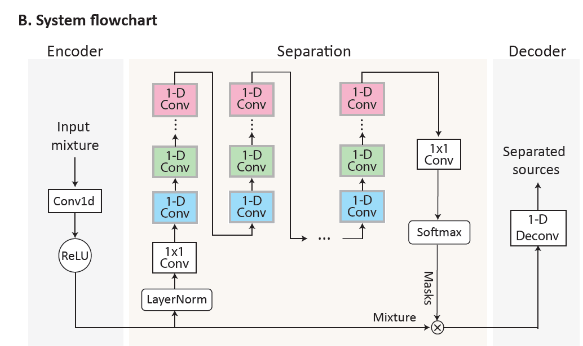
\includegraphics[scale=0.6]{obrazky-figures/tasnet-architecture.png}
    \caption{\label{fig:tasnet-modul}Schéma architektury TasNet}
\end{figure}

\blindtext{1}

\subsection{Konvoluční bloky}
- Z čeho se skládá -- konvoluční vrstvy, normalizace
- diagram konv bloku.
- Mozna: Dilatace a time perception
\begin{figure}[H]
    \centering
    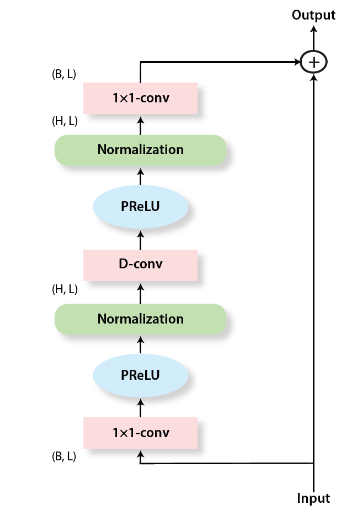
\includegraphics[scale=0.5]{obrazky-figures/conv-res-block.png}
    \caption{\label{fig:tasnet-convblock}Jeden konvoluční blok}
\end{figure}

\blindtext{1}

%----------------------------------------------------------------------------------------------------------------------------------------------------------------------



\chapter{Implementace a trénování sítě}
\label{implementace}
Pozn: colab, pytorch, stroj, bash, hyperparams, vykon a cas trenovani, seg--len, popis trid.

\section{Implementace modelu}
- pytorch, scripty, python3, bash, tridy, moduly, parametry a volby spusteni.

\section{Dataset}
\todo{Ukazat zde vykreslenou vlnu nahravek mix, s1, s2}
\todo{popsat co je dataset a k cemu to slouzi}
Trénování a vyhodnocení modelu proběhlo na množině jednokanálových nahrávek směsí dvou mluvčích. Množina byla vygenerována náhodným výběrem různých mluvčích z Wall Street Journal (WSJ0) a vytvořením směsi. Celková délka trénovacích dat je přes 10 hodin a přes 6 hodin validačních dat. Nahrávky jsou převzorkovány na 8kHz a během trénování zarovnány na zero means a jednotkovou varianci[studie str 5 Dataset][49 - ze studie odkaz na script na generovani a popis na netu].
\begin{figure}[H]
    \centering
    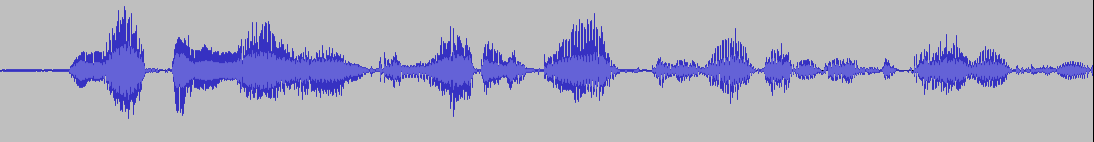
\includegraphics[scale=0.35]{obrazky-figures/dataset-mix.png}
    \caption{\label{fig:ref-mixture}Ukázka nahrávky směsi dvou mluvčích}
\end{figure}
\begin{figure}[H]
    \centering
    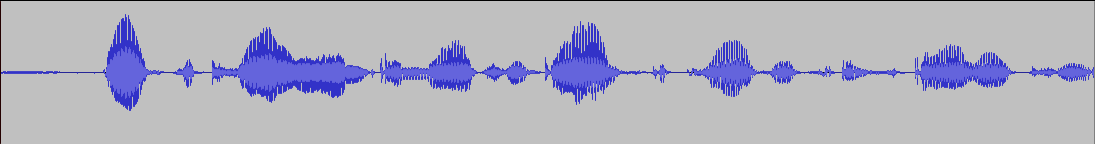
\includegraphics[scale=0.35]{obrazky-figures/dataset-s1.png}
    \caption{\label{fig:ref-s1}První mluvčí ze směsi}
\end{figure}
\begin{figure}[H]
    \centering
    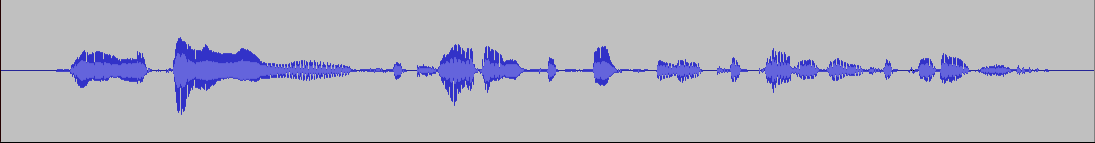
\includegraphics[scale=0.35]{obrazky-figures/dataset-s2.png}
    \caption{\label{fig:ref-s2}Druhý mluvčí ze směsi}
\end{figure}
Lze si všimnout, že sečtením signálů separovaných mluvčích na obrázku (ref obr1) a obrázku (ref obr2) dostaneme přesně signál směsi, což lze vyjádřit vztahem
\begin{equation}
  x(t) = \sum_{i=1}^C s_i(t)
\end{equation}
, kde $x(t) \in \mathbb{R}^{1 \times T}$ je diskrétní signál směsi a $s_i(t) \in \mathbb{R}^{1 \times T}$, kde $i = 1,\ldots,C$, je jeden z $C$ zdrojů[ref studie str3 vlevo]. 
\todo{doplnit info o zero means a jendotkove varianci}

\section{Trénování}
\begin{figure}[H]
    \centering
    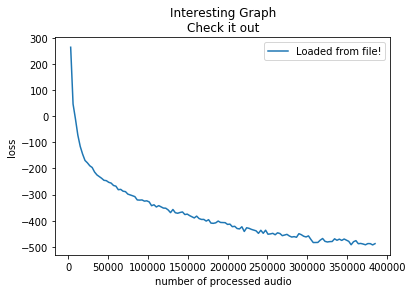
\includegraphics[scale=0.55]{obrazky-figures/some-loss.png}
    \caption{\label{fig:somelossTODO}Příklad grafu loss hodnoty během učení}
\end{figure}

\subsection{Význam validační množiny v trénování}
Většina algoritmů strojového učení má nějakou sadu hyperparametrů, kterou je upravováno chování algoritmu. Hodnoty hyperparametrů obvykle bývají nastavovány ručně ještě před spuštěním procesu učení a hodnota se v průběhu nemění, protože hodnoty by bylo obtížné optimalizovat. 
Některá nastavení se nicméně mohou stát hyperparametrem a být upravována během trénování, ale není vhodné je měnit na základě výsledku učení na trénovací sadě, protože by mohlo dojít k přetrénováníoverfitting) v důsledku \todo{CEHO??}. Pro tento případ potřebujeme validační sadu, která je odlišná od trénovací sady.
Po každém zpracování trénovací sady následuje validační sada, po jejímž skončení jsou optimalizovány hyperparametry[][].

\todo{[kniha 117-118] kap 5.3 = Hyperparameters and validation set} 
\todo{najit jeste nejakej zdroj s popisem a pripadne nejaky zajimavejsi info.}

\section{Vyhodnocovací metriky}
- minimalizovat objektivni-hodnotici funkci sisnr.
\subsection{Signal to noise ration}
\subsection*{Source Distortion Ratio -- SDR}
\subsection*{Artifacts Ratio -- SAR}
\subsection*{Inference Ratio -- SIR}



%----------------------------------------------------------------------------------------------------------------------------------------------------------------------


\chapter{Experimenty a vyhodnocení}
\label{experimenty}
- trenovani s ruznymi hyperparametry, uspesnost a tabulky s hyper parametry a dosazenymi vysledky a hodnotami sisnr, sdr atd.
- model size comparison.
- porovnani s vysledky ze studie
- obrazky separovanych mluvcich - signalu.
- spektra
- grafy trenovani loss a vysledkuu.
- pametova narocnost modelu


\section{Možná rozšíření a navrhnutá vylepšení}
- variabilnější dataset, mikrofony, šum a bordel prostředí
- separace více mluvčích
- hlučné prostředí
- identifikace konkrétního řečníka
- realtime separace

%----------------------------------------------------------------------------------------------------------------------------------------------------------------------

\chapter{Závěr}
\label{zaver}
- co jak dopadlo, vysledky a vyhodnoceni velikosti modelu a jaky byl nejlepsi,...
\blindtext[3]

